\begin{figure*}[p]
\centering
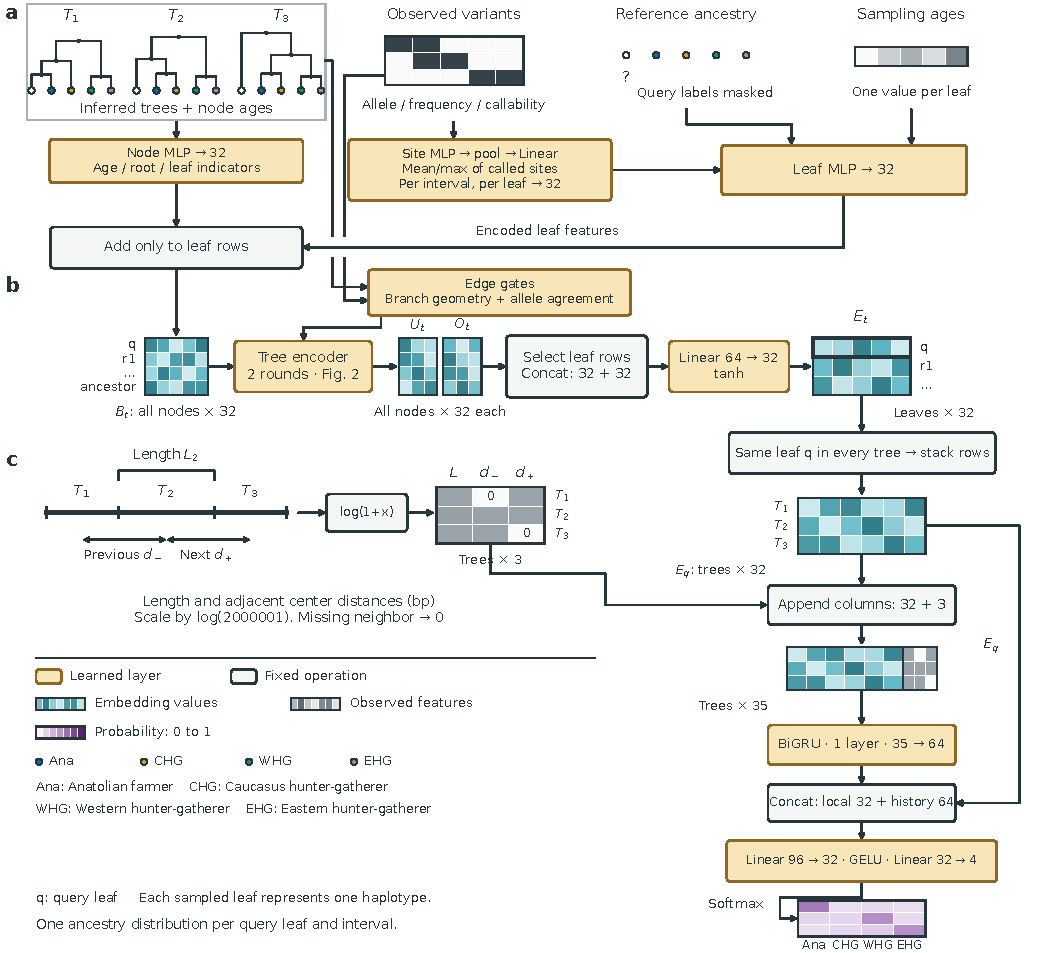
\includegraphics[width=\textwidth]{figures/TreeLoom_architecture.pdf}
\caption{\textbf{a,} Marginal trees, observed alleles and reference ancestry. The age cut defines descendant groups.
\textbf{b,} Two rounds each traverse complete trees upward then downward, sharing weights between rounds. Corrections $s$ and $\delta$ modify initial features before round 2. Figure~\ref{fig:operators} expands the node operations.
\textbf{c,} At the marked ancestor, $u+o$ projects to group context $f_2$. Copies enter separate forward and reverse tracks for r1 and r2. The inset expands each memory update. Directions and current group members are averaged, $f_2$ is subtracted, and projection gives $\delta$. History follows haplotypes when groups change. Other intervals' context inputs are omitted.
\textbf{d,} Query embeddings enter a BiGRU, classifier and softmax. The symbols $\parallel$, $\tfrac12\Sigma$ and $\times$ denote concatenation, averaging two vectors and scalar multiplication. Colors follow the legend. Values are illustrative.}
\label{fig:architecture}
\end{figure*}
